% Activate the following line by filling in the right side. If for example the name of the root file is Main.tex, write
% "...root = Main.tex" if the chapter file is in the same directory, and "...root = ../Main.tex" if the chapter is in a subdirectory.
 
%!TEX root =  

\chapter{Documentation}\label{doc}

\minitoc

This section provides documentation for the Privacy Advisor system. It gives an overview over the available documentation of source code, instructions for how to compile and install the system, and how it is used via. its GUI and command line interfaces.

\section{Source Code Documentation} 

The source code is documented using JavaDoc which is 	a tool that generates documentation in HTML format based on source code comments in Java, and is a standard part of the Java SDK. The JavaDoc for the Privacy Advisor system follows Sun Microsystems' style guide for writing JavaDoc comments\footnote{See: http://www.oracle.com/technetwork/java/javase/documentation/index-137868.html}. Source code documentation plays an important role in this project, as it is an early software prototype to be used in research which means that the code is then likely to be modified. The aim of the source code documentation is to supplement UML design documents to facilitate future development.

\section{Installation}

\subsection{Local Installation} \label{LocalInst}
To make the program run outside of the Eclipse environment it has to be exported as a runnable jar file. This can be done by right clicking the project in Eclipse, choose \texttt{Export}, type in \texttt{jar} in the new window that opens up and choose \texttt{Runnable Jar File}, before clicking \texttt{next}. These steps are shown in the two figures \ref{exportFirstStep} and \ref{exportSecondStep}.

  \begin{figure}
	\begin{centering}
    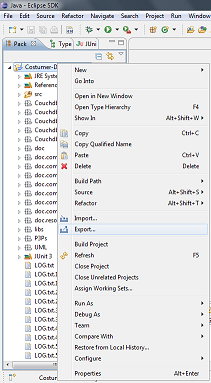
\includegraphics{Documentation/export.png}
    \caption{First step: right click and choose "export".}
    \label{exportFirstStep}
    \end{centering}
  \end{figure}


  \begin{figure}
  \begin{centering}
    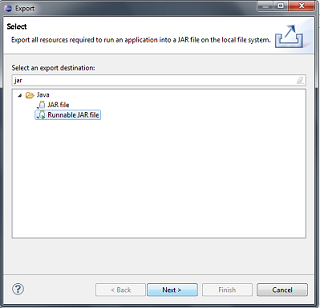
\includegraphics{Documentation/export_jar.png}
    \caption{Second step: choose runnable jar.}
    \label{exportSecondStep}
    \end{centering}
  \end{figure}


Then we have to choose which class file is to be the main class; in the \texttt{Launch configuration} dropdown menu we can choose between the two classes \texttt{PrivacyAdviser} and \texttt{PrivacyAdvisorGUI}. The first one is choosen if we want to run the program by using the command line, and the second one if we want to use the GUI. Then choose the export destination, and choose \texttt{Package requires libraries into generated JAR} as the library handling. Pressing finish now should start exporting the program. These steps are shown in figure \ref{exportLastStep}.


  \begin{figure}
\begin{centering}
    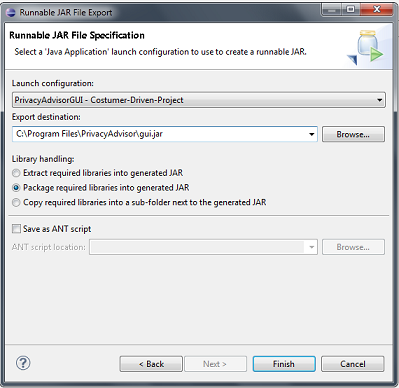
\includegraphics{Documentation/export_last.png}
    \caption{Third step: choose launch config, destination and library handling.}
    \label{exportLastStep}
\end{centering}
  \end{figure}


Before running the program we have to put the PrivacyAdviser.cfg file in the same folder as the exported jar file. And if the database file and the weights file isn't at the same folder, their location have to be specified in the PrivacyAdviser.cfg file. To run the program, open the command prompt and locate to the folder where the jar file is stored. Then write the command \texttt{java -jar filename.jar}, and now the program should start (even if it's the cli or gui version). This is shown in figure \ref{runProgram}.



  \begin{figure}
  \begin{centering}
    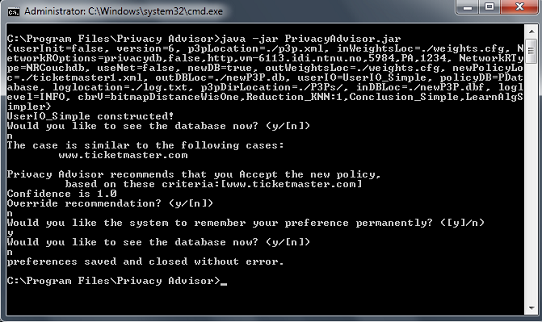
\includegraphics{Documentation/cli.png}
    \caption{Running the program.}
    \label{runProgram}
    \end{centering}
  \end{figure}


\subsection{Server Installation}
The CouchDB server is a default Ubuntu installation on a VMware virtual machine provided by NTNU IDI, with CouchDB installed using the command \texttt{sudo apt-get install couchdb}. The database server was configured via futon (the default web interface, located at localhost:5984\/\_util) to provide a database entitled \texttt{privacydb}, with a non-administration user (details noted in default program configuration file).

\section{User Interfaces}
The Privacy Adviser consist, as mentioned in section \ref{LocalInst}, of two different user interfaces. The advantage of the GUI is that it's easier to see the contents in the database before and after the program runs. The advantage of using the command line interface is that we can work much faster than by using the graphical user interface. But the best part of using the command line interface is that we can add options when calling (starting) the program, this is explained in detail in section \ref{cliExplained}.

\subsection{Command Line Interface} \label{cliExplained}
By running the program from the command line we can add options (parameters) directly when starting up the program. If we run the program normally, as described in section \ref{LocalInst}, the options in the PrivacyAdviser.cfg will be used. But when we add options in the command line when starting the program, the added options will override the ones in the config file.

As an example we can take the location of the database. By default the options in PrivacyAdviser.cfg is set to replace the old database with the new database when the program exits. There are two ways to change this. If we never or rarly want the new database to replace the old one we can just change the \texttt{outDBLoc} option to be different from the \texttt{inDBLoc} option in the config file. But if we want to change the location/name just once, we can add an option in the command line like this:
%put this in a box
\texttt{java -jar privacyAdvisor.jar -outDBLoc newDatabase.db}

We can add more than one option in this manner, and for the options that we don't specify, the options in the config file will be used. For a complete list of the options see table \ref{configTable}.

\subsection{Graphical User Interface}
When using the graphical user interface we can get an overview of the all the policies and cases in the database as a tree-structure. We can also see how the new policy that we want to add is structured. This can be seen in figure \ref{guiFigure}. The GUI is started from the command line the same way the CLI is started. When the GUI is stared, it automatically loads the database file, and displays the tree-structure. If we press the \texttt{Privacy Advisor} and  the \texttt{Run} buttons the process should start. If we want to change the location of the database, the new policy or anything else we can press the \texttt{Configuration} button and make the changes in the \texttt{Configuration Editor} window that shows up. This Configuration Editor window is showed in figure\ref{guiConfig}.

\begin{centering}
  \begin{figure}
    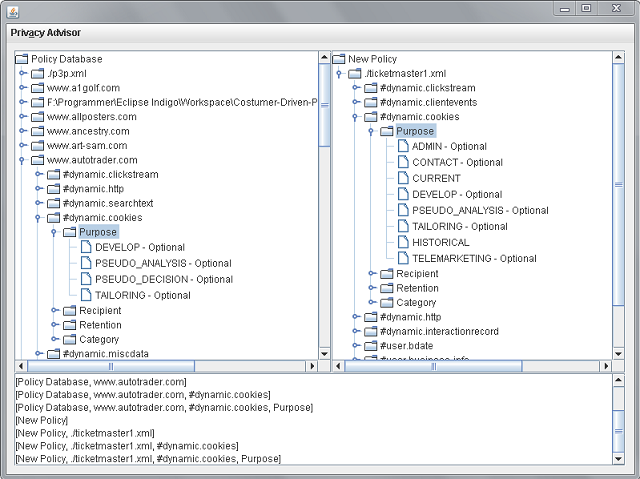
\includegraphics{Documentation/gui.png}
    \caption{The GUI.}
    \label{guiFigure}
  \end{figure}
\end{centering}

\begin{centering}
  \begin{figure}
    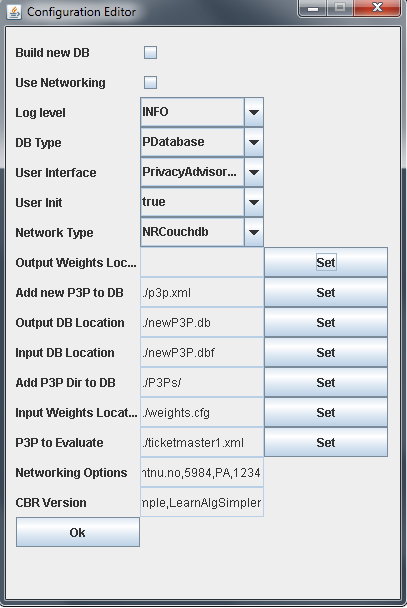
\includegraphics{Documentation/gui_config.png}
    \caption{Configuration in the GUI.}
    \label{guiConfig}
  \end{figure}
\end{centering}

\subsubsection{Configuration Files}

Table~\ref{configTable} gives an overview over the configuration file parameters.

\begin{center}
  \begin{table}[h!]
    \label{configTable}
    \begin{tabular} { | l | l | p{7cm} | }
      \hline
      \textbf{Item} & \textbf{Datatype} & \textbf{Description} \\ \hline
      loglocation & string/filepath  & where the log is written to. can't be changed once the UI is  called. \\ \hline
      loglevel & string/logging level	& what level to log at. \\ \hline
      inDBLoc & string/filepath	& where to read the past history from. \\ \hline
      outDBLoc & string/filepath & where to write DB- defaults to where it reads from. \\ \hline
      inWeightsLoc& string/filepath & where to read the weights config file from. \\ \hline
      outWeightsLoc	& string/filepath & where to write DB- defaults to where it reads from. \\ \hline
      newDB & string/boolean & are we overwriting/ignoring an old database. \\ \hline
      p3pLocation & string/filepath & a p3p to be added to the history. \\ \hline
      p3pDirLocation	& string/FOLDERpath& a folder of p3ps to be added to the history. \\ \hline
      blanketAccept & string/boolean & accept the advisers recommendation. \\ \hline
      newPolicyLoc & string/filepath	& the new policy to be parsed. \\ \hline
      userInit & string/boolean	& true if some initialization occurs via the user interface. \\ \hline
      userResponse & string/action	& the response to the suggestion, if know beforehand. \\ \hline
      cbrV & string/CBR & parses for algorithms, etc to use. See CBR:parse(String). \\ \hline
      userIO & string/UIO	& the user interface to use. see Gio:selectUI. \\ \hline
      policyDB & string/policyDB & select the database type. see Gio:selectPDB . \\ \hline
      genConfig	& string/filepath & load an alternate configuration file. \\ \hline
      networkRType & string/classname & the name of a networkR class. \\ \hline
      networkROptions & string/commasepoptions	& the options necessary for the above networkR class. \\ \hline
      confidenceLevel & string/double & the confidence level at which the algorithm trusts itself; if below this, it uses the server's suggestion. \\ \hline
      useNet & string/boolean & whether to activate network functionality. \\ \hline
      \hline
    \end{tabular}
    \caption{Configuration file parameters.}
  \end{table}
\end{center}

\subsubsection{Building a Database}

\textbf{CLI}: To build a new database from a directory \texttt{P3PDir} holding P3P files, Privacy
Advisor can be called from the command line in the following fashion:
\texttt{PrivacyAdvisor -newDB  true -outDBLoc new.db
  -p3pDirLocation P3PDir}.

\textbf{GUI}: To build a new database in the similar fashion using the
graphical user interface, the configuration window can be set up
similarly to that illustrated in figure[XXXX].



\subsubsection{Loading and Viewing a Database}



\subsubsection{Parsing a P3P Policy}
